% ЕМТ 2025, IX клас — точен LaTeX препис от официалните файлове в Klasirane.com.
% Условия: https://klasirane.com/api/competitions/EMT/All/2025/9%20%D0%BA%D0%BB/probs
% SHA-256 (условия): c8b57f70fc90fb83ab4c0ef849d3011e5ff7e122ff7a920894a8091c0d67ce44
% Решения: https://klasirane.com/api/competitions/EMT/All/2025/9%20%D0%BA%D0%BB/sol
% SHA-256 (решения): 793feb2b7ab8e4fe529648dab779a9dfca98e39a7a612edbf122197e6a299e35
% Точковите оценки, правописът и формулировките са запазени от източника.
% Файлът с условията е едностранично сканирано изображение; видимата страница е проверена пряко.
% Файлът с решенията продължава със задача 10.1 след решение 9.4; този препис спира в края на IX клас.

Задача 9.1. Уравнението $x^2+ax+b=0$ има два корена $x_1$ и $x_2$, които са естествени числа и за които е изпълнено равенството:

$$\frac{x_1+20}{x_1-20}=\frac{x_2+26}{x_2-26}.$$

Да се намери най-малката стойност на $b$.

Решение. Привеждаме под общ знаменател.

$$(x_1+20)(x_2-26)=(x_1-20)(x_2+26)$$

$$x_1x_2+20x_2-26x_1-20\cdot26=x_1x_2-20x_2+26x_1-20\cdot26$$

Съкращаваме и получаваме $10x_2=13x_1$. Най-малките естествени числа, които удовлетворяват това равенство са $x_1=10$ и $x_2=13$. Тъй като $b=x_1x_2=\frac{10}{13}x_2^2$, а най-малката стойност на $b$ се получава при най-малката стойност на $x_2$, то $b=130$.

Оценяване. 1 т. за премахване на знаменателя; 1 т. за опростяване; 2 т. за най-малкото решение в естествени числа; 2 т. за довършване.

Задача 9.2. Точките $P$ и $Q$ са от страната $AB$ (в ред $A$, $P$, $Q$ и $B$), а точката $R$ е от страната $BC$ на триъгълник $ABC$. Отсечката $AR$ пресича отсечките $CP$ и $CQ$ съответно в точки $X$ и $Y$. Ако $APYC$ и $PQYX$ са вписани четириъгълници и $\angle ACB=70^\circ$, да се намери ъгълът между правите $QX$ и $BC$.

Решение. Тъй като $PQXY$ е вписан имаме $\angle XPQ+\angle XYQ=180^\circ$. Тогава:

$$(1)\qquad \angle APX+\angle CYX=(180^\circ-\angle XPQ)+(180^\circ-\angle XYQ)=180^\circ.$$

Сега от вписания четириъгълник $APYC$ получаваме $\angle APX=\angle CYX$ и от (1) намираме $\angle APX=\angle CYX=90^\circ$, т.е. $X$ е ортоцентър за $\triangle AQC$. Следователно $QX\perp AC$ и от $\angle ACB=70^\circ$ получаваме, че търсеният ъгъл е $20^\circ$.

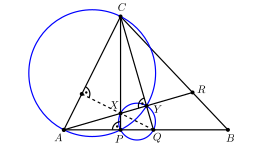
\includegraphics[max width=0.46\textwidth, alt={Официалната фигура към решение 9.2 с триъгълника ABC и точките P, Q, R, X и Y}, center]{assets/9-2-geometry.svg}

Оценяване. 2 т. за $\angle APX=90^\circ$ или $\angle CYX=90^\circ$; 2 т. за намиране, че $X$ е ортоцентър за $\triangle AQC$; 2 т. за довършване.

Задача 9.3. Да се реши в цели неотрицателни числа уравнението $x^3+16=y^2$.

Решение. Първо да отбележим че $(0,4)$ е решение. Да разгледаме остатъците на $y^2$ и $x^3$ по модул 9. Директно проверяваме, че в първия случай те са $0,1,4,7$ а във втория — $0,1,8$. Тъй като $16\equiv-2\pmod 9$, значи $y^2\equiv7\pmod 9$ и $x\equiv0\pmod 9$. Следователно $x=3z$ за някое цяло $z$.

Получаваме $27z^3=(y-4)(y+4)$. Значи или $y-4$ се дели на 27 или $y+4$ се дели на 27.

1сл. $y=27k+4$. Тогава $27z^3=27k(27k+8)$. Нека $g=\gcd(27k,27k+8)$. Тъй като степента на 2 трябва да е кратна на 3, имаме $g=1,8$.

Ако $g=1$, тогава $27k=u^3$ и $27k+8=w^3$. Но тогава $u^3+8=w^3$ няма решение. Ако $g=8$, тогава $27z^3=64(27k_1)(27k_1+1)$ и аналогично на предния случай ще стигнем до $u^3+1=w^3$. Тогава $k_1=0$, следователно $z=0$, $x=0$ и стигаме до известното решение.

2 сл. $y=27k-4$. Имаме $27z^3=27k(27k-8)$ и можем да приложим точно същият анализ.

Окончателно получаваме че други решения няма.

Оценяване. 2 т. за остатъците на квадратите по $\mod 9$; 1 т. за кратността на $x$; 1 т. за представянето $27z^3=(y-4)(y+4)$, 2 т. за 1 сл., 1 т. за довършване.

Бележка: Този тип диофантови уравнения се наричат уравнения на Мордел, а кривите от вида $y^2=x^3+ax+b$ се наричат елиптични криви и имат редица важни приложения.

Задача 9.4. В равнината са дадени 101 прави $l_1,l_2,\ldots,l_{101}$ в общо положение (всеки две се пресичат и никои три не минават през една точка). Върху пресечната точка на правите $l_i$ и $l_j$ е записано числото $i+j$.

Множество $A$ от $k$ естествени числа е такова, че върху всяка права е записано поне едно число от $A$ и ако махнем произволно число от $A$ съществува права, върху която няма записано число от новото множество. Да се намерят всички възможни стойности на $k$.

Решение. Ще докажем, че възможните стойности са $k=2,3,4$.

Ако $k=1$, то $A=\{a\}$ и при $a\le101$ върху правата 101 няма число, при $a=102$ върху правата 51 няма число и при $a\ge103$ върху правата 1 няма число.

При $k=2$ множеството $A=\{102,52\}$ е хубаво.

При $k=3$ множеството $A=\{105,4,3\}$ е хубаво.

При $k=4$ множеството $A=\{106,108,6,4\}$ е хубаво.

Нека $k\ge5$. Ясно е, че или има три числа $a<b<c\le101$ или има три числа $102\le m<n<p$.

Нека $a<b<c\le101$. Ще покажем, че на всички прави, на които се среща числото $a$ се среща някое от числата $b$ или $c$. Нека на права $x$ се среща числото $a$. Следователно съществува $y$, за което $x+y=a$. Тогава $x+(b-x)=b$ и $x+(c-x)=c$, като $101>b>b-x>a-x=y\ge1$ и $101\ge c>c-x>a-x=y\ge1$. Тъй като $x=b-x$ и $x=c-x$ не са възможни едновременно, то поне в единия сбор $x+(b-x)=b$ и $x+(c-x)=c$ двете събираеми са различни. Това означава, че на правата $x$ се среща едно от числата $b$ или $c$.

Нека $102\le m<n<p$. Ще покажем, че на всички прави, на които се среща числото $p$ се среща някое от числата $m$ или $n$. Нека на права $x$ се среща числото $p$. Следователно съществува $1\le y\le101$, за което $x+y=p$. Тогава $x+(m-x)=m$ и $x+(n-x)=n$, като $1\le m-x<p-x=y\le101$ и $1\le n-x<p-x=y\le101$. Тъй като $x=m-x$ и $x=n-x$ не са възможни едновременно, то поне в единия сбор $x+(m-x)=m$ и $x+(n-x)=n$ двете събираеми са различни. Това означава, че на правата $x$ се среща едно от числата $m$ или $n$.

И в двата случая получихме противоречие, което означава че възможните стойности са $k=2,3,4$.

Оценяване. 2 т. за примери и за трите стойности за $k$ (1 т. за примери за две от възможните стойности за $k$); 3 т. за доказване, че не може да има три числа по-малки от 102 (или три числа по-големи от 101); 5 т. за доказване и на двете твърдения.
